\chapter {Implementacja}
\label{cha:implementacja}
Poniższy rozdział przedstawia aspekty implementacyjne projektu. Na wstępie omówiono użyte technologie oraz narzędzia wraz z uzasadnieniem wyboru. Następnie przedstawiono dokładny model aplikacji z uwzględnieniem wybranych technologii implementacyjnych. 
W rozdziale tym przedstawiono także problemy implementacyjne, z którymi zetknęli się autorzy oraz sposoby ich rozwiązania.
\section {Wybrane technologie i narzędzia}
Przed przystąpieniem do implementacji końcowej wersji aplikacji powstawały prototypy testujące różne podejścia algorytmiczne opisane w rozdziale \ref{cha:Algorytm} oraz możliwe do wykorzystania narzędzia. W sekcji \textit{Język implementacji} przedstawiono język wybrany do implementacji końcowej wersji programu, natomiast w sekcji \textit{Języki prototypowania} przedstawiono technologie używane do tworzenia prototypów systemu.
\subsection{Język implementacji}
Jednym z pierwszych pytań, na które należy odpowiedź podejmując się implementacji systemu jest język programistyczny wykorzystywany do jego implementacji. W przypadku projektu Sparkle do implementacji końcowej wersji aplikacji został wybrany język Java.
Język ten został wybrany ze względu na łatwą przenośność aplikacji, obiektowość ułatwiającą projektowanie, łatwy dostęp do licznych 
bibliotek oraz mechanizmy pozwalające uchronić program przed wyciekami pamięci krytycznymi z punktu widzenia aplikacji czasu rzeczywistego. Innym, rozważanym językiem implementacji był C++. Przed końcowym wyborem zostały przeprowadzone badania dotyczące wydajności rozważanych języków. Przyniosły one następujące rezultaty:
%http://java.sun.com/docs/performance/ - może z tego uda się coś wyciągnąć o efektywności javy
\begin{itemize}

\end{itemize}

\subsection{Języki prototypowania}
Jednym z powstałych ptotypów był prosty automat komórkowy z regułami opisanymi w paragrafie [WSTAWIC ODNOSNIK DO PARAGRAGU].Do implementacji tego modelu został korzystany język Lisp.
\\\\
[TUTAJ WSTAWIC ZALETY LISPA DO PROTOTYPOWANIA - WYMYSLISZ COS PRAWDA :>?]
\\
Drugim, powstałym podczas badań pierwowzorem był program napisany w języku Java.
Celem tego modelu było przetestowanie języka Java oraz biblioteki Java3D pod kątem możliwości wykorzystania do implementacji symulacji czasu rzeczywistego w oparciu o uproszczony model automatu. 

\subsection {Moduł wizualizacji}
Wizualizacja symulacji została zaimplementowana z wykorzystaniem Java3D API.
Java3D to interfejs programowy (API) umożliwiający tworzenie trójwymiarowej grafiki. Jest to produkt firmy Sun Microsystems wykorzystujący w swoim działaniu renderery OpenGL i Direct3D w zależności od platformy.
Główną zaletą determinująca wybór bilioteki Java3D jest umożliwienie wykorzystania technologii OpenGL i DirectX poprzez dostarczenie wysokopoziomowych struktur pozwalających zachować pełnię obiektowości języka Java. 
Zastosowana w bibliotece Java3D obiektowość ułatwia zarządzanie elementami sceny oraz umożliwia skupienie uwagi na logice aplikacji bez zagłębiania się w szczegóły renderingu. Inną niezmiernie ważną zaletą biblioteki Java3D jest optymalizacja procesów renderingu.
\subsubsection{Instalacja biblioteki Java3D}
Instalacja biblioteki Java3D jest bardzo prosta i może przebiegać na dwa sposoby.
Pierwszym sposobem jest ściącienie ze strony https://java3d.dev.java.net/binary-builds.html archiwum zip. Po jego rozpakowaniu należy, postępując zgodnie z instrukcją zawartą w pliku README-unzip.html, zmodyfikować zmienną CLASSPATH dodając ścieżki do wymienionych w instrukcji plików z rozszrzeniem .jar oraz zmodyfikować zmienną PATH dodając ścieżkę do katalogu lib\i386.


Alternatywą jest pobranie ze strony firmy Oracle http://www.oracle.com/technetwork/java/javase/tech/index-jsp-138252.html
instalatora, który pod dwukrotnym kliknięciu przeprowadzi użytkownika przez proces instalacyjny. 
W wyniku instalacji Java Runtime Environment System Library zostanie wzbogacone o pliki j3dcore.jar i j3dutils.jar.
\subsubsection{Budowa sceny z wykorzystaniem struktur Java3D API}
Głównym elementem biblioteki Java3D jest graf sceny (\textit{scene graph}) rerezentujący cały wirtualny wszechświat (\textit{virtual universe}). Graf sceny jest acyklicznym grafem skierowanym.  Użytkownik tworzy podgrafy reprezentujące pewne wycinki rzeczywistości, które następnie są dołączane jako dzieci do wirtualnego wrzechświata. Kazdy z podgrafów jest renderowany  osobno i niezależnie od pozostałych, co pozwala na zrównoleglenie obliczeń. Strukturę grafu sceny przedstawia diagram \ref{java3d_diagram_sceny}.
\begin{figure}
\begin {center}
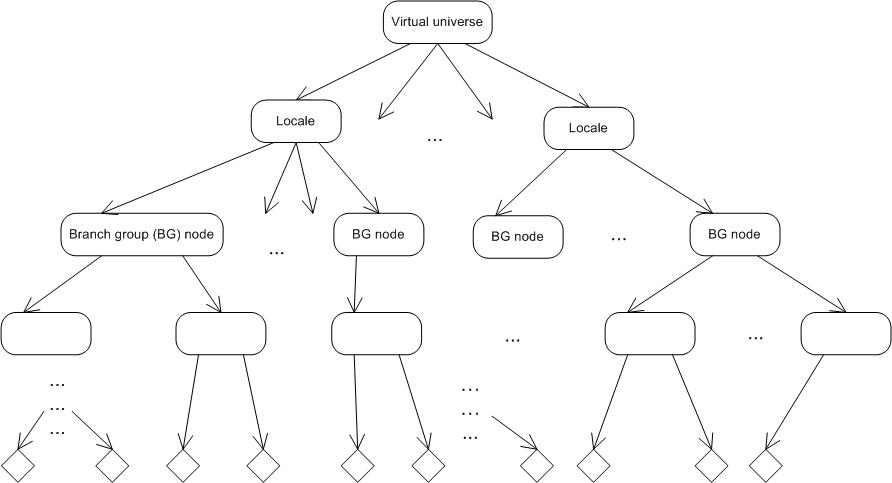
\includegraphics{java3d_diagram_sceny.jpg} 
\caption {Java3D - reprezentacja sceny}
\label {java3d_diagram_sceny}
\end {center}
\end{figure}
 Wśród jego wierzchołków możemy wyróżnić:
\begin{itemize}
\item Group nodes - wierzchołki reprezentujące grupę elementów. Mogą zawierać zero lub więcej dzieci. Grupowanie elementów umożliwia wykonywanie operacji dla całej grupy. Na diagramie \ref{java3d_diagram_sceny} przedstawione są jako zaokrąglone kształty.
\item Leaf nodes - liście reprezentują obiekt tworzący scenę (geometrię, oświtlenie, dźwięk). Nie mogą posiadać dzieci. Na diagramie \ref{java3d_diagram_sceny} występują w postaci rombów.
\end{itemize}
Korzeniem całego grafu jest obiekt klasy \textit{VirtualUniverse} lub dowolnej, dziedziczącej po niej klasie. Graf sceny może posiadać wiele wierzchołków, jednak w większości przypadków jeden jest wystarczający. Obiekt klasy \textit{Locale} jest kontenerem przechowującym kolekcję podgrafów, których korzeniami są instancje klasy \textit {BranchGroup}. Obiekt klasy \textit{BranchGroup} powinien być postrzegany jako jednostka, która po stworzeniu jest kompilowana, a następnie dołączana do grafu reprezentującego wirtualny wszechświat. W dowolnym momencie może zostać odłączana i powtórnie dołączona w inne miejsce.
Tworzenie obiektu 3D przy użyciu Java3D API przebiega następująco:
\begin{enumerate}
\item Tworzony jest obiekt. Ustalane są jego właściwości.
\item Stworzony obiekt dołączany jest do odpowiedniego grafu reprezentowanego przez obiekt BranchGroup.
\item Powstałe grafy w ten sposób grafy są łączone w jedną strukturę reprezentującą wirtualny wszechświat.
\end{enumerate}
Dobrą praktyką jest wspomniane powyżej kompilowanie stworzonych podgrafów przed ich połączeniem. Nie jest ono konieczne ale powoduje  zamianę grafu do wewnętrznego formatu umożliwiającego jego optymalizację. Na uwagę zasługuje fakt, że domyślnie obiekty mogą być modyfikowane jedynie podczas tworzenia podgrafu. Po dołączeniu już stworzonego podgrafu do większej całości informacja o jego obiektach jest oddzielnie zapamiętywana, w sposób przyspieszający operacje dostępu do danych. Można to zmienić wywołując podczas tworzenia obiektu metodę \textit{setCapability} z odpowiednim parametrem.

\subsection {Narzędzia pracy grupowej}
Ze względu na fakt, że omawiana aplikacja powstała jako wynik pracy dwuosobowego zespołu bardzo przydatnym narzędziem okazał się system kontroli wersji. Jako system zarządzania wersjami został wybrany Git.
Git jest darmowym, rozproszonym systemem, opartym na architekturze peer-to-peer. W przeciwieństwie do scentralizowanych odpowiedników (np. SVN) nie posiada jednego, centralnego repozytorium z którym członkowie zespołu synchronizują swoje zmiany ale wiele niezależnych gałęzi, które można synchronizować w różnorodny sposób. Główną zaletą systemu Git, będącą motywacją jego wyboru...






